\subsection{Phân tích và thiết kế hệ thống}

\subsubsection{Kiến trúc Dataware house}
\begin{enumerate}
    \item \textbf{Kiến trúc cũ:}
    \begin{center}
            \begin{figure}[!h]
                \centering
                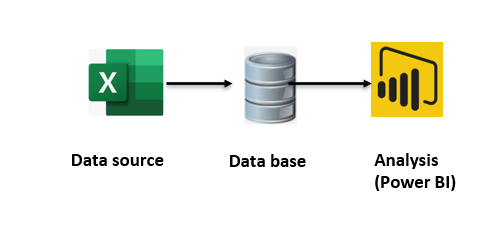
\includegraphics[scale = 1]{figures/Duyen/Kiến trúc cũ.PNG}
              \caption{Kiến trúc DW cũ}
            \end{figure}
\end{center}
    Mô hình cũ thực hiện các hoạt động phân tích dữ liệu ngay trên hệ thống lưu trữ. Điều này đem lại một số hạn chế như:
    \begin{itemize}[label=$-$]
        \item Làm giảm hiệu năng hệ thống 
\item Dữ liệu để phân tích không ổn định
\item Tốc độ xử lý chậm.
    \end{itemize}
Chính vì thế ta cần xây dựng mô hình mới để khắc phục được những hạn chế này:
    \item \textbf{ Kiến trúc mới:}\\
Đặc điểm hệ thống mới:
Sử dụng kiến trúc có vùng Staging, trong đó:
\begin{itemize}
    \item Nguồn dữ liệu là file CSV chứa dữ liệu thô.
    \item Vùng Staging là khu vực lưu trữ trung gian được sử dụng để thực hiện các bước ETL dữ liệu, ví dụ như xử lý dữ liệu Null, dữ liệu đa trị, định dạng kiểu dữ liệu, tách thành các bảng,...
    \item Data Warehouse là nơi dữ liệu được lưu trữ và quản lí để phục vụ cho việc phân tích thống kê, báo cáo, khai thác và trực quan hóa dữ liệu.
    \item Lớp phân tích được sử dụng để đưa ra các báo cáo và dashboard theo các chủ đề đã nêu thông qua một số công cụ trực quan hoá dữ liệu.
    
\end{itemize}\newpage
    \begin{center}
            \begin{figure}[!h]
                \centering
                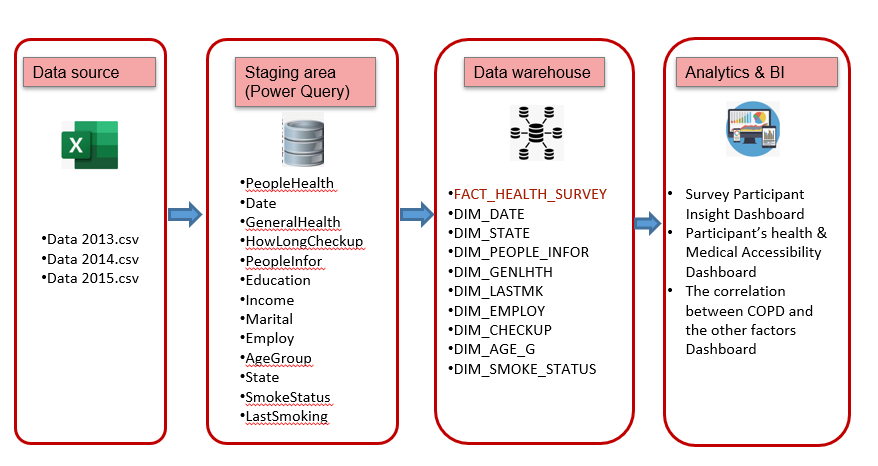
\includegraphics[scale = 0.8]{figures/Duyen/Kiến trúc mới.PNG}
              \caption{Kiến trúc DW mới}
            \end{figure}
\end{center}
\end{enumerate}

\newpage
\subsubsection{Data Exploration}
Thông tin của người thực hiện khảo sát
\begin{itemize}[label=$-$]
\item  Tỷ lệ giới tính 
\begin{center}
            \begin{figure}[!h]
                \centering
                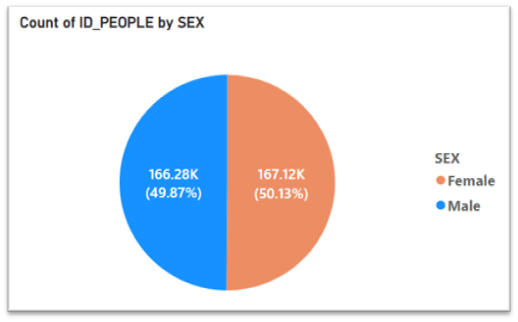
\includegraphics[scale = 0.8]{figures/Hoa/DE1.1.png}
              \caption{Tỷ lệ giới tính}
            \end{figure}
\end{center}
\begin{itemize}[label=$+$]
\item Từ biểu đồ ta thấy tỷ lệ giới tính của số người tham gia khảo sát là gần như ngang nhau : với tỷ lệ "Male" chiếm 49.78\% và tỷ lệ "Female" chiếm 50.13\%.
\end{itemize}

\item Độ tuổi tham gia khảo sát 
\begin{center}
            \begin{figure}[!h]
                \centering
                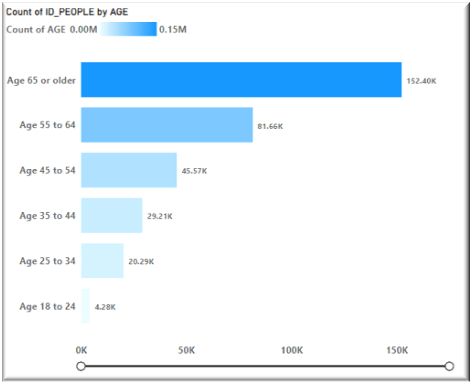
\includegraphics[scale = 0.8]{figures/Hoa/DE1.2.png}
              \caption{Độ tuổi tham gia khảo sát}
            \end{figure}
\end{center}
\begin{itemize}[label=$+$]
\item Ở khảo sát này thì có chia làm 6 nhóm tuổi và bắt đầu từ 18 tuổi trở lên.
\item Nhìn vào biểu đồ ta có thể thấy số lượng người tham gia khảo sát ở độ tuổi 65 tuổi trở lên rất cao lên đến 152.40K người, và số lượng người tham gia giảm dần theo chiều giảm của độ tuổi. Điều này cho thấy càng lớn tuổi con người càng có xu hướng quan tâm đến sức khỏe bản thân nhiều hơn.
\end{itemize}
\item Tình trạng việc làm 
\begin{center}
            \begin{figure}[!h]
                \centering
                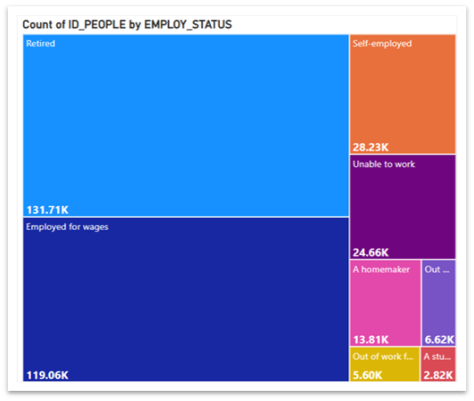
\includegraphics[scale = 0.8]{figures/Hoa/DE1.3.png} 
              \caption{Tình trạng việc làm }
            \end{figure}
\end{center}
\begin{itemize}[label=$+$]
\item Cũng tương tự như Độ tuổi tham gia khảo sát, có số lượng người từ 65 tuổi trở lên chiếm đa số thì tình trạng việc làm tương ứng là "Retired" ( Đã nghỉ hưu) cũng chiếm đa số, lên đến 131.71K người.
\item Số lượng người làm công ăn lương cũng chiếm một phần không nhỏ lên đến 119.06K người và ít nhất là học sinh, sinh viên.
\end{itemize}
\newpage
\item Tình trạng hôn nhân
\begin{center}
            \begin{figure}[!h]
                \centering
                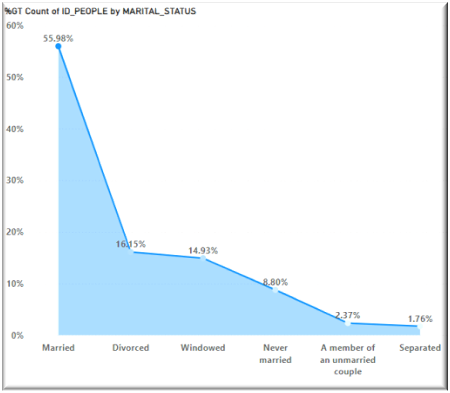
\includegraphics[scale = 0.7]{figures/Hoa/DE1.4.png} 
              \caption{Tình trạng hôn nhân }
            \end{figure}
\end{center}
\begin{itemize}[label=$+$]
\item Tình trạng hôn nhân của người tham gia khảo sát được chia thành 6 nhóm : Đã kết hôn, Đã ly hôn , Góa vợ hoặc chồng, Không bao giờ kết hôn, Chưa kết hôn, Ly thân.
\item Trong đó tỷ lệ người đã kết hôn chiếm đến 55.98\% điều đó cũng do hầu hết người được khảo sát từ 18 tuổi trở lên và phần lớn mọi người đã đủ khả năng để kết hôn.
\end{itemize}
\item Mức thu nhập
\begin{center}
            \begin{figure}[!h]
                \centering
                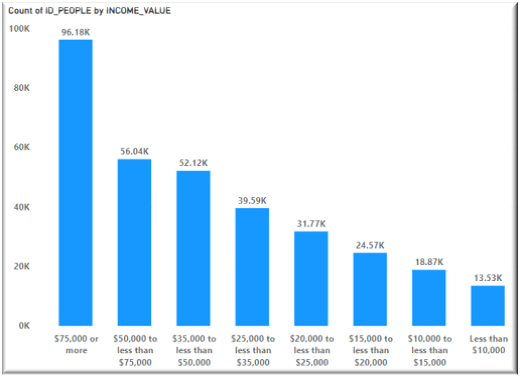
\includegraphics[scale = 0.7]{figures/Hoa/DE1.5.png} 
              \caption{Mức thu nhập }
            \end{figure}
\end{center}
\begin{itemize}[label=$+$]
\item Mức thu nhập được chia thành 8 nhóm trải dài từ ít hơn \$10.000 đến nhiều hơn \$75000.
\item Số người có mức thu nhất \$75.000 hoặc lớn hơn chiếm đa số lên đến 96.18K người, và giảm dần theo chiều giảm của mức thu nhập. Điều đó cho ta thấy phần lớn người tham gia khảo sát có thu nhập khá cao 
\end{itemize}
\end{itemize}
Khả năng tiếp cận y tế
\begin{itemize}[label=$-$]
\item Tỷ lệ người có bảo hiểm y tế
\begin{center}
            \begin{figure}[!h]
                \centering
                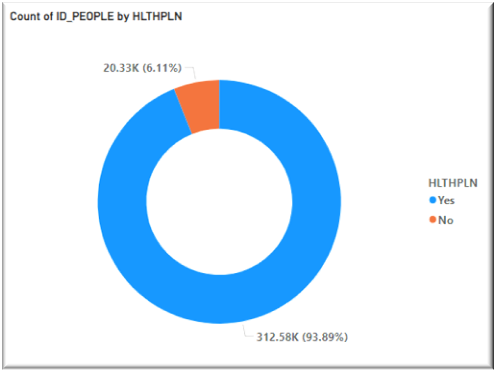
\includegraphics[scale = 0.9]{figures/Hoa/DE2.1.png} 
              \caption{Bảo hiểm y tế }
            \end{figure}
\end{center}
\begin{itemize}[label=$+$]
\item Số lượng người có bảo hiểm y tế lên đến 312.58K chiếm đến 93.89\%, điều này hoàn toàn phù hợp với mức thu nhập cao của số người tham gia khảo sát.
\item Tuy nhiên vẫn còn đến 20.33K người chưa có bảo hiểm y tế, cho thấy khả năng tiếp cận y tế của họ vẫn chưa cao.
\end{itemize}\newpage
\item Tỷ lệ giữa các khoảng thời gian chưa đi kiểm tra sức khỏe theo từng  khu vực
\begin{center}
            \begin{figure}[!h]
                \centering
                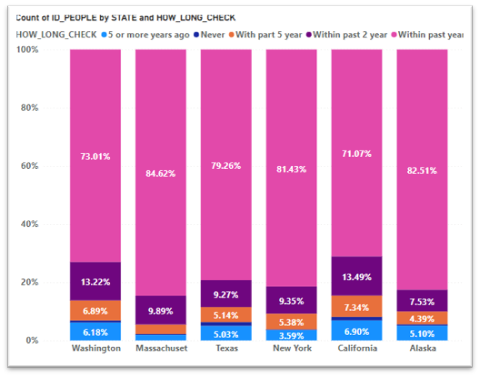
\includegraphics[scale = 0.8]{figures/Hoa/DE2.2.png} 
              \caption{Thời gian đi kiểm tra sức khỏe }
            \end{figure}
\end{center}
\begin{itemize}[label=$+$]
\item Thời gian đi kiểm tra sức khỏe được chia làm 4 nhóm theo độ dài của thời gian.
\item Ta có thể thấy phần lớn mọi người đi kiểm tra sức khỏe trước đó chưa đến 1 năm 
\item Bên cạnh đó vẫn có nhiều người khám sức khỏe trước đó 2 năm, 5 năm và thậm chí là nhiều hơn 5 năm.
\end{itemize}
\item Số người có bác sĩ riêng theo từng khu vực
\begin{center}
            \begin{figure}[!h]
                \centering
                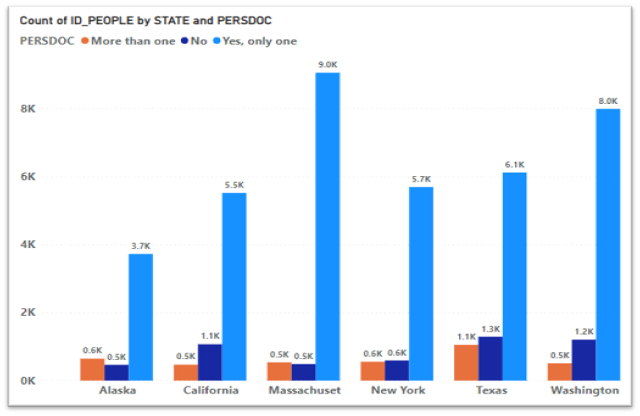
\includegraphics[scale = 0.6]{figures/Hoa/DE2.3.png} 
              \caption{Bác sĩ riêng }
            \end{figure}
\end{center}
\begin{itemize}[label=$+$]
\item Nhìn vào báo cáo ta có thể thấy, phần lớn người tham gia khảo sat có 1 bác sĩ riêng, và cũng có một phần người có nhiều hơn 1 bác sĩ riêng.
\item Có một phần người tham gia khảo sát không có bác sĩ riêng, họ là những người có mức thu nhập thấp và có khả năng tiếp cận y tế thấp.
\end{itemize}
\end{itemize}
Thực trạng của việc hút thuốc lá
\begin{itemize}[label=$-$]
\item Số người sử dụng thuốc lá theo từng nhóm tuổi
\begin{center}
            \begin{figure}[!h]
                \centering
                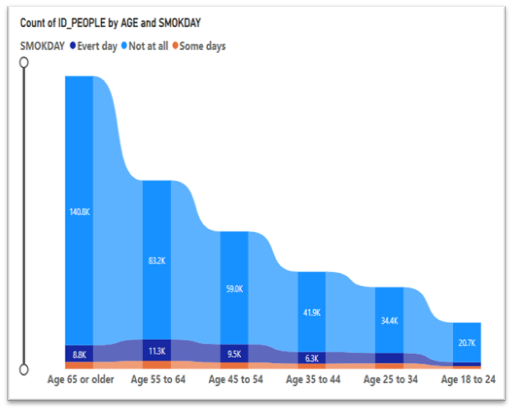
\includegraphics[scale = 0.9]{figures/Hoa/DE3.1.png} 
              \caption{Theo độ tuổi }
            \end{figure}
\end{center}
\begin{itemize}[label=$+$]
\item Biểu đồ cho thấy phần lớn người tham gia khảo sát không hút thuốc lá
\item Nhưng vẫn có một bộ phận người hút thuốc lá hàng ngày và cao nhất ở nhóm tuổi từ 55 đến 64.
\end{itemize}\newpage
\item Tình trạng hút thuốc lá ở từng khu vực 
\begin{center}
            \begin{figure}[!h]
                \centering
                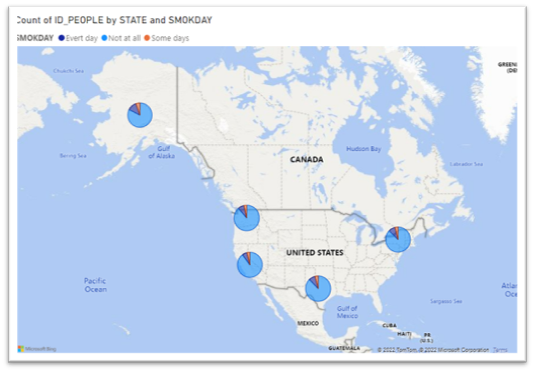
\includegraphics[scale = 0.9]{figures/Hoa/DE3.2.png} 
              \caption{Theo khu vực }
            \end{figure}
\end{center}
\begin{itemize}[label=$+$]
\item Tỉ lệ hút thuốc lá ở các khu vực là gần như nhau, phần lớn mọi người đều không sử dụng thuốc lá.
\end{itemize}
\end{itemize}\newpage

\subsubsection{ETL}

Dữ liệu gốc chứa gần 1,5 triệu bản ghi các dữ liệu đều đã được mã hóa dưới dạng số. Tha thực hiện ETL dữ liệu bằng Excel  gồm các thao tác như thay thế giá trị , đổi kiểu dữ liệu , tách cột , xử lý các cột ngày tháng 
Đầu tiên đưa dữ liệu vào Power query .Nhận thấy có 3 file dữ liệu của năm 2013 , 2014, 2015 đều có các cột tương ứng giống nhau . Để giúp cho việc thống kê và báo cáo được dễ dàng hơn  ta thực hiện nối các bảng lại với nhau bằng cách sử dụng \textit{Append Quieries } .\\
\\\textbf{Xử lý dữ liệu mã hóa }\\
Các dữ liệu trong bảng 2013, 2014,2015 đều đã được mã hóa dưới dạng số. Do đó cần phải giải mã chúng để đưa về các giá trị cụ thể chi tiết hơn. Có rất nhiều cách để giải mã như tách cột, thêm cột, thêm cột có
điều kiện, thay thế giá trị, .... Cụ thể:
\begin{itemize}
    \item Giải mã dữ liệu cột IDAY , IMONTH , IYEAR \\\hfill
    Nhận thấy dữ liệu trong các cột \textit{IDAY, IMONTH ,IYEAR} đều được bao bọc bởi cặp dấu \textbf{''} do đó cần phải tách dữ liệu ra bằng cách xử dụng \textit{Split Column } với dấu phân cách là \textbf{'}. Ta thu được kết quả khi tách cột \textit{IMONTH} như hình dưới :\\
    
            \begin{figure}[!h]
                \begin{center}
                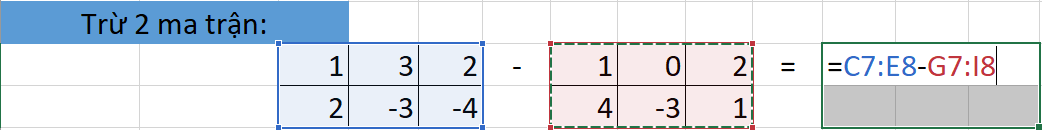
\includegraphics[scale = 0.8]{HONG/2.png}
              \caption{Tách dữ liệu cột IMONTH}
         
\end{center}
   \end{figure}
   Sau khi đã tách dữ liệu của 3 cột ta thực hiện xóa các cột \texit{IMONTH.1,IMONTH.3 , IYEAR.1 ,IYEAR.3 ,IDAY.1 ,IDAY.3 }bởi vì các cột này đều không có giá trị sử dụng . Thực hiện gộp các cột \textit{ IDAY.2 , IMONTH.2 ,IYEAR.2  }  với nhau bằng cách sử dụng\textit{ merge columns} với seperator là / , sau đó chuyển dữ liệu về dạng ngày tháng ta thu được kết quả như hình dưới đây :
    \begin{figure}[!h]
                \begin{center}
                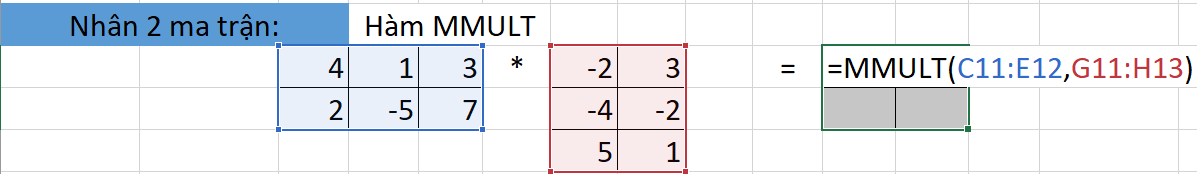
\includegraphics[scale = 0.8]{HONG/3.png}
              \caption{Merge quieres}
         
\end{center}
   \end{figure}
   \item Giải mã hóa các cột giá trị khác \\\hfill
   Thực hiện thay thế các giá trị số thành các giá trị cụ thể ví dụ như ở cột \textbf{SEX} chỉ có 2 giá trị số là 1 và 2 , nhìn vào giá trị ta không thể biết được nó có nghĩa là gì do đó ta cần giải mã nó với 1 tương ứng là\textit{ male} , với 2 tương ứng là\textit{ female }.
   Thực hiện giải mã bằng cách thay thế giá trị (sử dụng replace values ) hoặc megre quieres bảng gốc với bảng dữ liệu giải mã tương ứng . Tuy nhiên khi dữ liệu bị mã hóa có nhiều việc thay thế giá trị sẽ rất là tốn thời gian do đó ta thực hiện merge quieres thu được kết quả như hình dưới
     \begin{figure}[!h]
                \begin{center}
                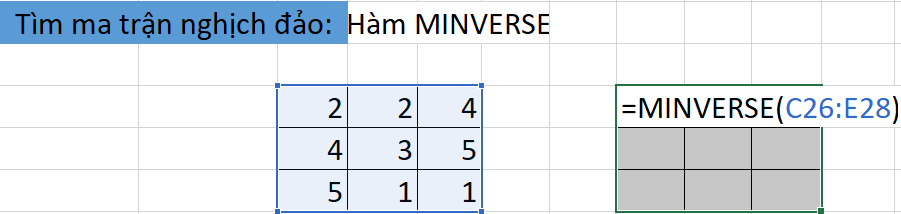
\includegraphics[scale = 0.8]{HONG/5.png}
                \caption{Merge quieres}
                \end{center}
    \end{figure}
\end{itemize}
\textbf{Xóa các giá trị \textit{NULL} trong bảng }\\
Thực hiện xóa các giá trị \textit{NULL} ở mỗi bảng .Các giá trị này sẽ làm cho việc báo cáo thống kê phức  tạp do đó ta cần thực thao tác xóa . Dưới đây là kết quả của quá trình xóa các giá trị null trong cột \textbf{LASTSMK2} :
 
            \begin{figure}[!h]
                \begin{center}
                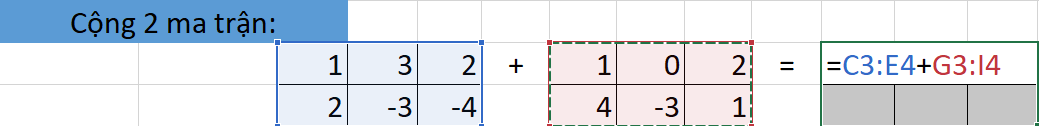
\includegraphics[scale = 0.7]{HONG/1.png}
              \caption{Xóa giá trị NULL cột LASTSMK2}
         
\end{center}
   \end{figure}


Ngoài ra để tiện cho việc truy vấn dữ liệu  ta có thể lưu dữ liệu vào cơ sở dữ liệu:\\
\begin{itemize}
    \item Dữ liệu sau khi được xử lí đơn giản được lưu vào CSDL HealthCare, vùng dữ liệu
được lưu này gọi là Stagging, là vùng đệm chứa dữ liệu trước khi đưa vào kho dữ liệu.
\item Xây dựng kho dữ liệu bằng cách tạo các bảng trong cơ sở dữ liệu theo mô hình OLAP
đã được thiết kế.

\end{itemize}
Đổ dữ liệu từ cơ sở dữ liệu vào kho dữ liệu bằng cách sử dụng SQL Server Import and Export Wizard trong SQL sever:\newpage
\begin{center}
            \begin{figure}[!h]
                \centering
                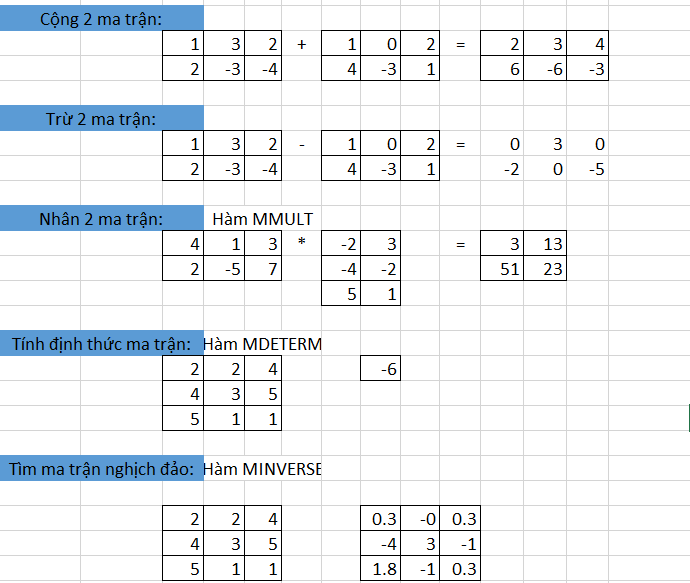
\includegraphics[scale = 0.9]{HONG/6.png} 
              \caption{IMPORT DATA}
            \end{figure}
\end{center}
\begin{itemize}
    \item Các dữ liệu cố định, không thay đổi theo thời gian sẽ được chuyển trực tiếp từ Stagging vào Kho dữ liệu thông qua câu lệnh “Insert” như bên dưới :
    \begin{center}
            \begin{figure}[!h]
                \centering
                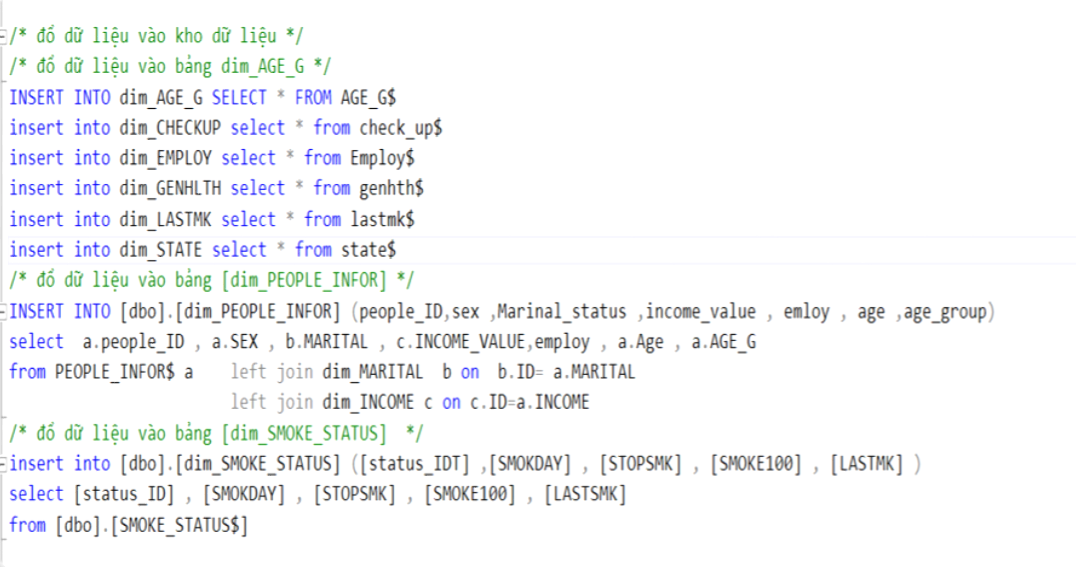
\includegraphics[scale = 0.6]{HONG/8.png} 
              \caption{Câu lệnh INSERT}
            \end{figure}
\end{center}
\item Đối với các dữ liệu được cập nhật định kì theo thời gian (tức là cứ sau một khoảngthời gian sẽ có dữ liệu) mới được thêm vào thì việc cứ mỗi lần  phải viết lại câu lệnh “Insert” là rất mất thời gian. Thay vào đó, ta sẽ đưa câu lệnh “Insert” tạo thành một thủ tục để mỗi lần cập nhật dữ liệu ta chỉ cần gọi thủ thục một cách nhanh chóng:
\begin{center}
            \begin{figure}[!h]
                \centering
                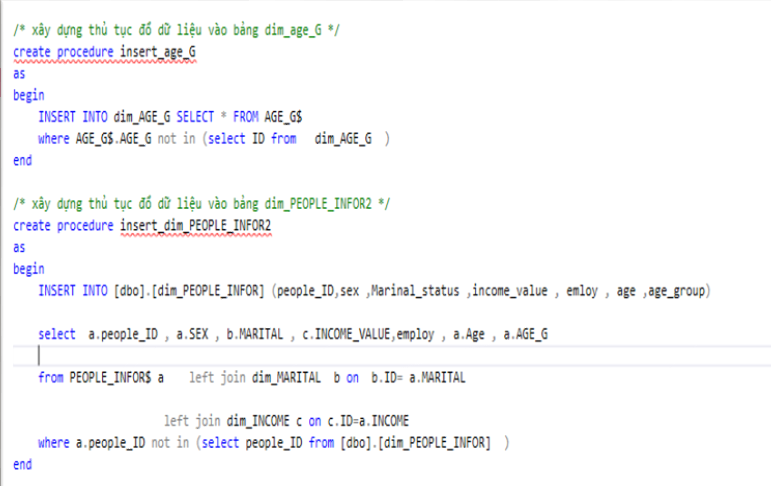
\includegraphics[scale = 0.75]{HONG/9.png} 
              \caption{Thủ tục INSERT}
            \end{figure}
\end{center}
Sau khi đã xây dựng xong các thủ tục ta thử kiểm tra lại kết quả :
\begin{center}
            \begin{figure}[!h]
                \centering
                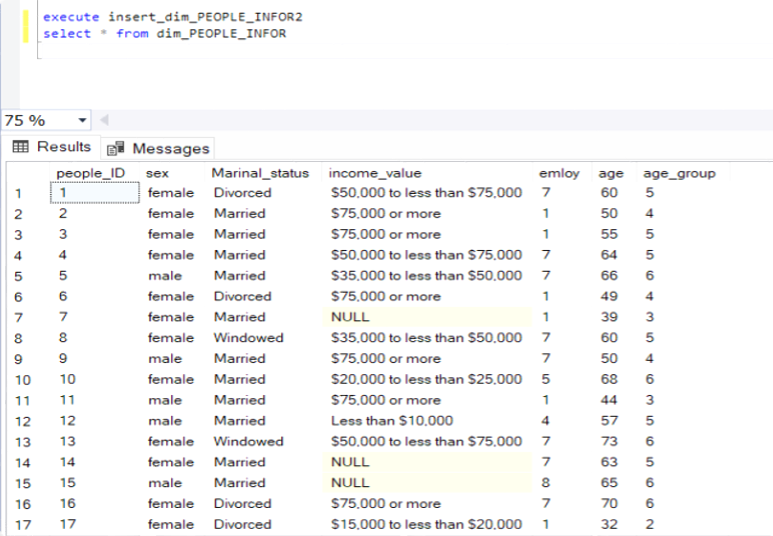
\includegraphics[scale = 0.75]{HONG/10.png} 
              \caption{Kết quả}
            \end{figure}
\end{center}
\end{itemize}
\newpage
\subsubsection{Facts}
Chủ điểm phân tích của hệ thống được mô tả trong bảng "FACT\_HEALTH\_SURVEY" với khoá chính là SURVEY\_ID và 4 khoá phụ bao gồm: PEOPLE\_ID, REGION\_ID, DATE\_ID, STATUS\_ID cùng với thuộc tính CHCCOPD.
\begin{center}
            \begin{figure}[!h]
                \centering
                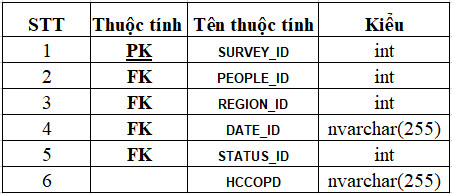
\includegraphics[scale = 0.9]{van/fact.png} 
              \caption{FACT\_HEALTH\_SURVEY}
            \end{figure}
\end{center}

\subsubsection{Dimension}
Theo chủ điểm phân tích FACT\_HEALTH\_SURVEY" ta có các chiều phân tích theo thời gian, tính trạng sức khoẻ, thông tin của người tham gia khảo sát, tình trạng hút thuốc và khu vực.
\begin{itemize}
    \item Chiều về thời gian\\
    Chiều về thời gian bao gồm thời gian tham gia khảo sát với khoá chính là DATE\_ID.
    \begin{center}
            \begin{figure}[!h]
                \centering
                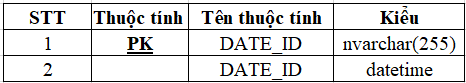
\includegraphics[scale = 0.8]{van/dim_date.jpg}
              \caption{OLAP DIM\_DATE}
            \end{figure}
    \end{center}
    \item Chiều về tình trạng sức khoẻ của người tham gia khảo sát\\
    Có khoá chính là PEOPLE\_ID và 7 thuộc tính lần lượt là: HEALTH\_STATUS, HLTHPLN, PERSDOC, MEDCOST, HOW\_LONG\_CHECKUP, WEIGHT\_KG, HEIGHT\_CM.
    \begin{center}
            \begin{figure}[!h]
                \centering
                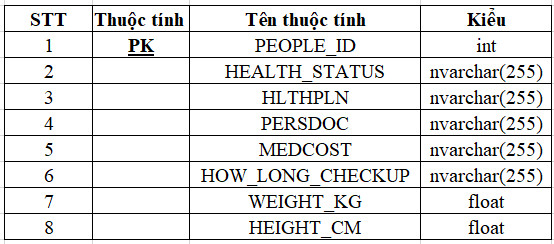
\includegraphics[scale = 0.8]{van/oltp dim heath.png}
              \caption{OLAP DIM\_HEALTH}
            \end{figure}
    \end{center}
    \item Chiều về thông tin người tham gia khảo sát\\
    Được phân cấp thành 3 bảng như sau:
    \begin{center}
            \begin{figure}[!h]
                \centering
                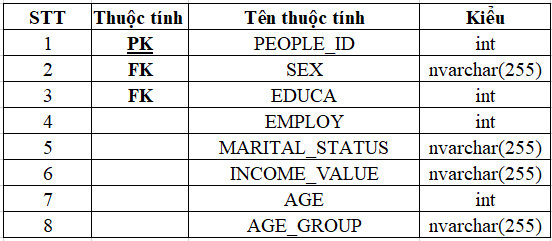
\includegraphics[scale = 0.8]{van/olap dim people infor.png}
              \caption{OLAP DIM\_PEOPLE\_INFOR}
            \end{figure}
    \end{center}
    \begin{center}
            \begin{figure}[!h]
                \centering
                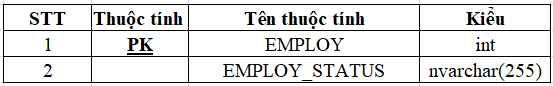
\includegraphics[scale = 0.8]{van/olap dim employ.jpg}
              \caption{OLAP DIM\_EMPLOY}
            \end{figure}
    \end{center}
    \begin{center}
            \begin{figure}[!h]
                \centering
                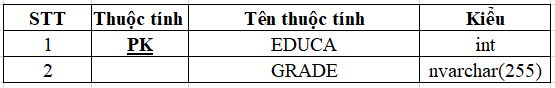
\includegraphics[scale = 0.8]{van/olap dim education.jpg}
              \caption{OLAP DIM\_EDUCATION}
            \end{figure}
    \end{center}
    \item Chiều về tình trạng hút thuốc của người tham gia khảo sát\\
    Gồm một khoá chính STATUS\_ID và 5 thuộc tính: SMOKEDAY, STOPSMK, SMOKE100, HOW\_LONG\_LAST\_SMOKE, USENOW.
    \begin{center}
            \begin{figure}[!h]
                \centering
                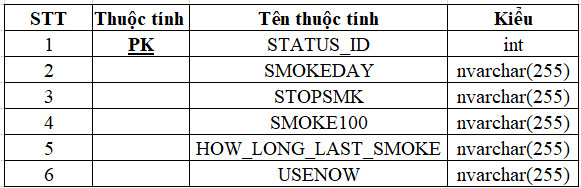
\includegraphics[scale = 0.8]{van/olap dim smoke status.png}
              \caption{OLAP DIM\_SMOKE\_STATUS}
            \end{figure}
    \end{center}
    \item Chiều về địa điểm khu vực khảo sát\\
    Gồm một khoá chính REGION\_ID và thuộc tính STATE.
    \begin{center}
            \begin{figure}[!h]
                \centering
                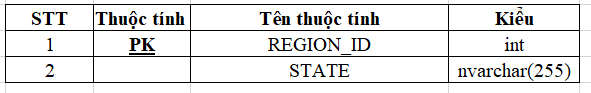
\includegraphics[scale = 0.8]{van/olap dim region.png}
              \caption{OLAP DIM\_SMOKE\_STATUS}
            \end{figure}
    \end{center}
\end{itemize}
\newpage
Sau đây là phần thống kê dữ liệu theo các chiều:
\begin{itemize}
    \item Chiều về thời gian
    \begin{center}
            \begin{figure}[!h]
                \centering
                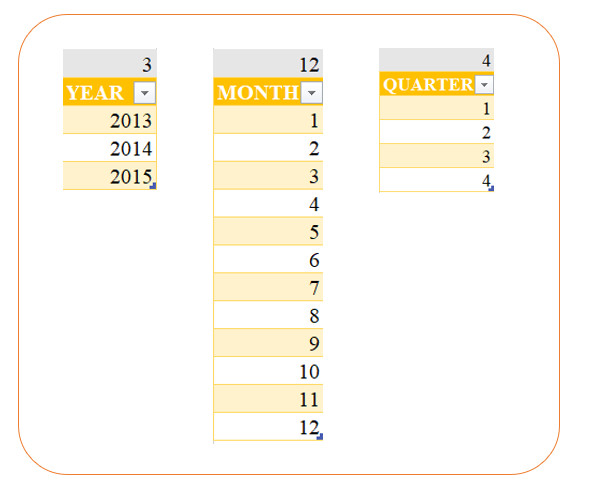
\includegraphics[scale = 0.6]{van/dim_tg.png}
              %\caption{OLAP DIM\_SMOKE\_STATUS}
            \end{figure}
    \end{center}
    \item Chiều về tình trạng sức khoẻ người tham gia khảo sát
    \begin{center}
            \begin{figure}[!h]
                \centering
                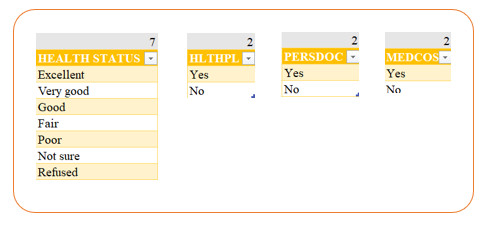
\includegraphics[scale = 0.6]{van/dim_sk.png}
              %\caption{OLAP DIM\_SMOKE\_STATUS}
            \end{figure}
    \end{center}
    \newpage 
    \item Chiều về khu vực
    \begin{center}
            \begin{figure}[!h]
                \centering
                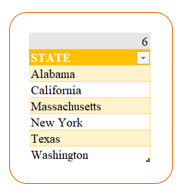
\includegraphics[scale = 0.6]{van/dim_kv.png}
              %\caption{OLAP DIM\_SMOKE\_STATUS}
            \end{figure}
    \end{center} 
    \item Chiều về tình trạng hút thuốc của người tham gia khảo sát 
    \begin{center}
            \begin{figure}[!h]
                \centering
                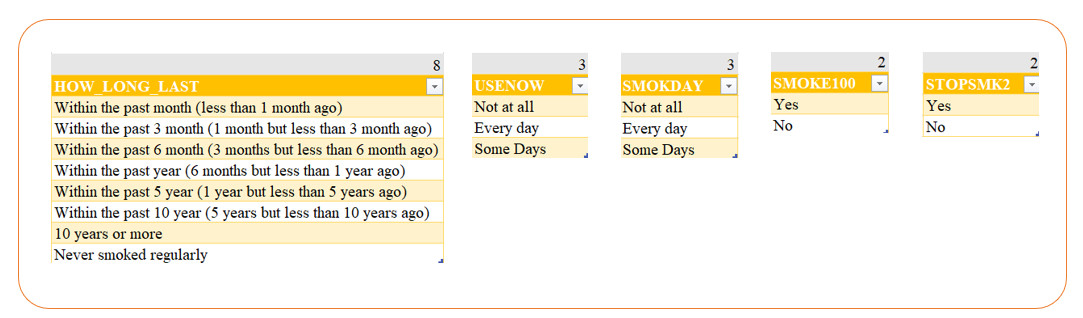
\includegraphics[scale = 0.4]{van/dim_tt.png}
              %\caption{OLAP DIM\_SMOKE\_STATUS}
            \end{figure}
    \end{center}
    \item Chiều về thông tin người tham gia khảo sát
    \begin{center}
            \begin{figure}[!h]
                \centering
                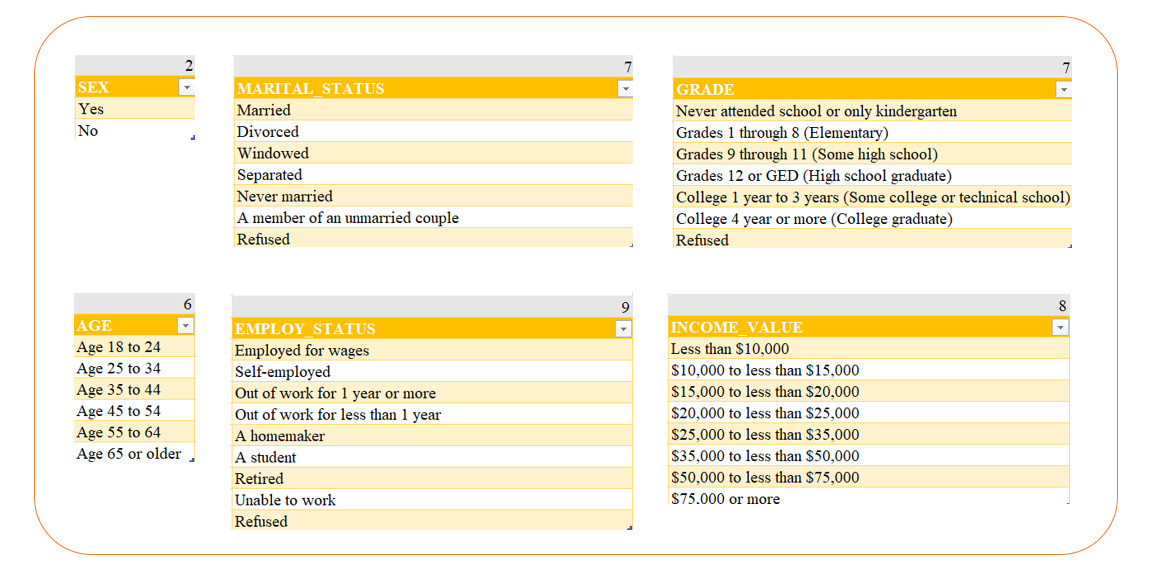
\includegraphics[scale = 0.4]{van/dim_inf.png}
              %\caption{OLAP DIM\_SMOKE\_STATUS}
            \end{figure}
    \end{center}
    
\end{itemize}

\subsubsection{Data model-ERD}
\begin{center}
            \begin{figure}[!h]
                \centering
                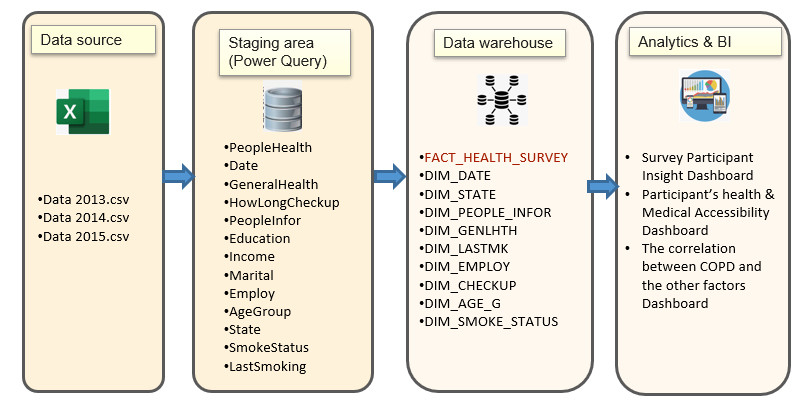
\includegraphics[scale = 0.4]{van/oltp healthcare.png}
              \caption{Kiến trúc hệ thống OLAP Healthcare}
            \end{figure}
    \end{center}
    Tầng dưới cùng là hệ CSDL quan hệ “DataCo\_OLTP”. Các công cụ đầu cuối, các tiện ích được dùng để đưa dữ liệu vào tầng dưới cùng từ hệ cơ sở dữ liệu hoạt động hoặc từ nguồn bên ngoài (file csv, excel...). Những công cụ và tiện ích này thực hiện việc loạibỏ dữ liệu thừa, làm sạch dữ liệu, chuyển đổi dữ liệu, cập nhật dữ liệu. Dữ liệu được lưu trữ vào 13 bảng: 
    
\begin{itemize}
    \item PEOPLEHEALTH
    \item DATE
    \item GENARALHEALTH
    \item HOWLONGCHECKUP
    \item PEOPLEINFOR
    \item EDUCATION
    \item INCOME
    \item MARITAL
    \item EMPLOY
    \item AGEGROUP
    \item STATE
    \item SMOKESTATUS
    \item LASTSMOKING
\end{itemize}

Tầng giữa là Data warehouse “DataCo\_OLAP” được cài đặt dùng mô hình quan hệ OLAP. Dữ liệu được đổ từ mô hình OLTP của hệ CSDL hoạt động sang mô hình OLAP của Data warehouse, bao gồm các bảng:
\begin{itemize}
    \item FACT\_HEALTH\_SURVEY
    \item DIM\_HEALTH
    \item DIM\_DATE
    \item DIM\_REGION
    \item DIM\_PEOPLE\_INFOR
    \item DIM\_EDUCATION
    \item DIM\_EMPLOY
    \item DIM\_SMOKE\_STATUS
\end{itemize}
Tầng trên cùng là tầng người dùng cuối, gồm các câu truy vấn và các công cụ làm báo cáo, phân tích, công cụ khai thác dữ liệu về:
\begin{itemize}
    \item Survey Participant Insight Dashboard: thông tin chi tiết người tham gia khảo sát.
    \item Participant’s health \& Medical Accessibility Dashboard: tổng quan về khả năng tiếp cập y tế và sức khỏe người tham gia khảo sát.
    \item The correlation between COPD and the other factors Dashboard: mối tương quan giữa COPD và các yếu tố khác.
\end{itemize}
\newpage
\subsubsection{Data model OLAP}
Mô hình logic
\begin{center}
        \begin{figure}[!h]
            \centering
            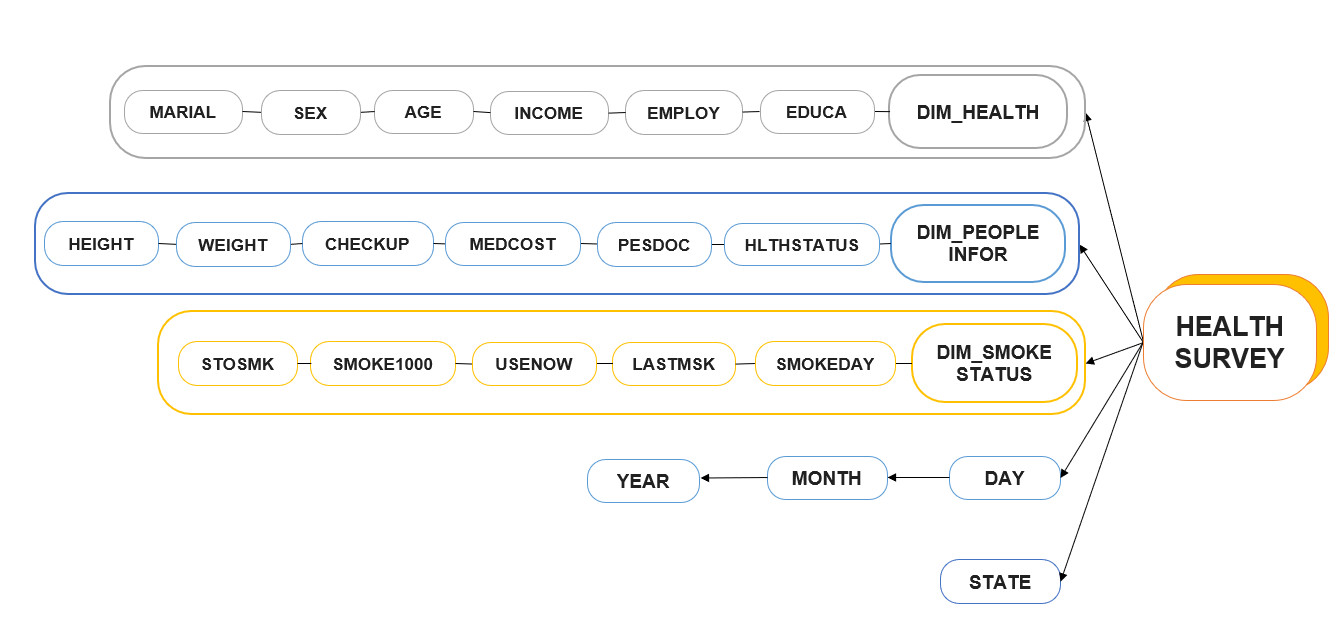
\includegraphics[scale = 0.35]{van/oltp_logic.png}
             \caption{Mô hình logic của hệ thống OLAP}
        \end{figure}
\end{center}

Mô hình quan hệ
\begin{center}
        \begin{figure}[!h]
            \centering
            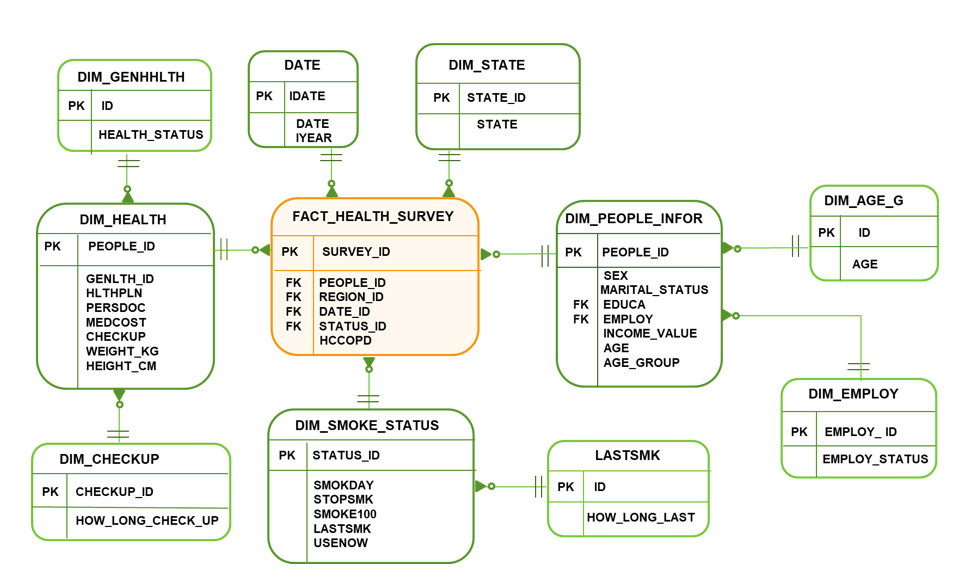
\includegraphics[scale = 0.4]{van/oltp_erd.png}
             \caption{Mô hình quan hệ của hệ thống OLAP}
        \end{figure}
\end{center}
    







